\subsection{Additional functions}

\begin{frame}{Additional functions: graphical summary}
    \begin{itemize}
        \item \textbf{Box-plot:} graphical summary of the distribution of simulations results
    \end{itemize}
    \textbf{}
    \begin{figure}[t]
        \centering
        \textbf{compositionPop2()}\par\medskip
        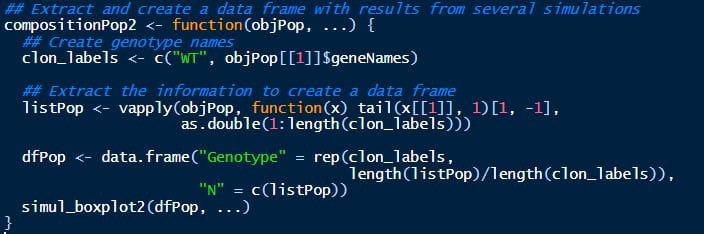
\includegraphics[width=0.9\linewidth]{img/compositionPop2.PNG}
        \caption{Code for compositionPop2() function}
    \end{figure}
\end{frame}

\begin{frame}{Additional functions: graphical summary}
    \begin{figure}[t]
        \centering
        \textbf{simul\_boxplot2()}\par\medskip
        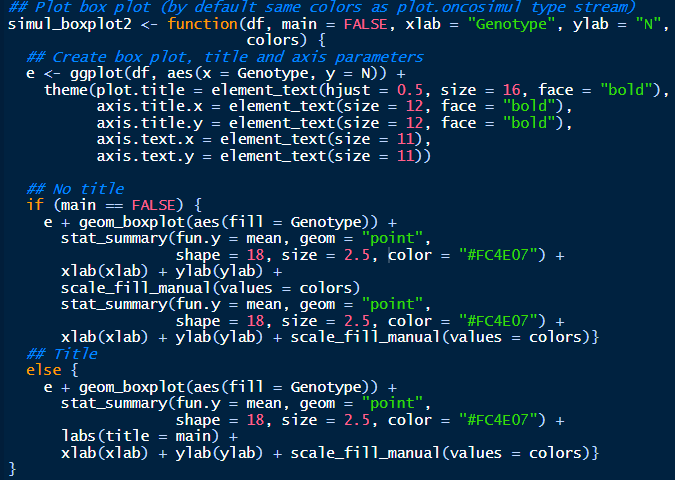
\includegraphics[width=0.65\linewidth]{img/simul_boxplot.PNG}
        \caption{Code for simul\_boxplot2() function}
    \end{figure}
\end{frame}

\begin{frame}{Additional functions: graphical summary}
    \begin{figure}
    \centering
    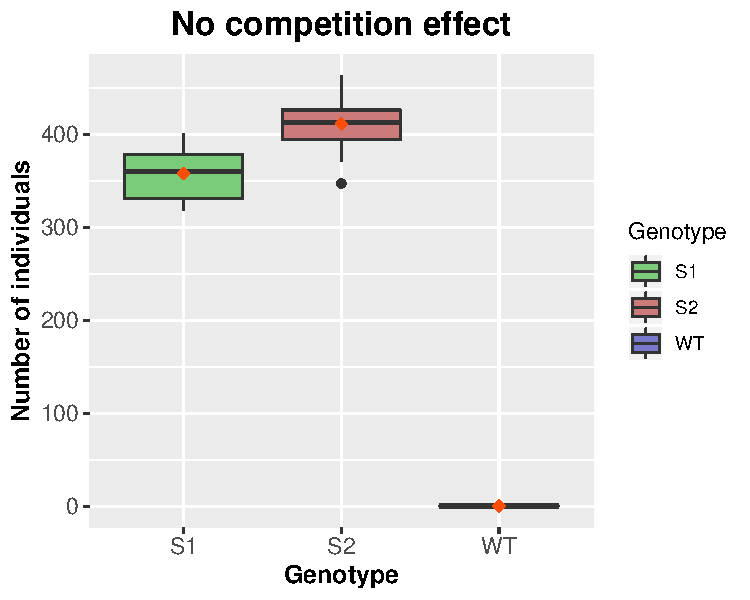
\includegraphics[width=0.65\linewidth]{img/boxplot_example.pdf}
    \caption{Box-plot from one of the Lotka-Volterra's example. 20 simulations were made}
    \end{figure}
\end{frame}

\begin{frame}{Additional functions: graphical summary}
    \begin{itemize}
    \item \textbf{Stripchart:} summary of simulations with oscillating trajectories
     \end{itemize}
     \begin{figure}
        \centering
        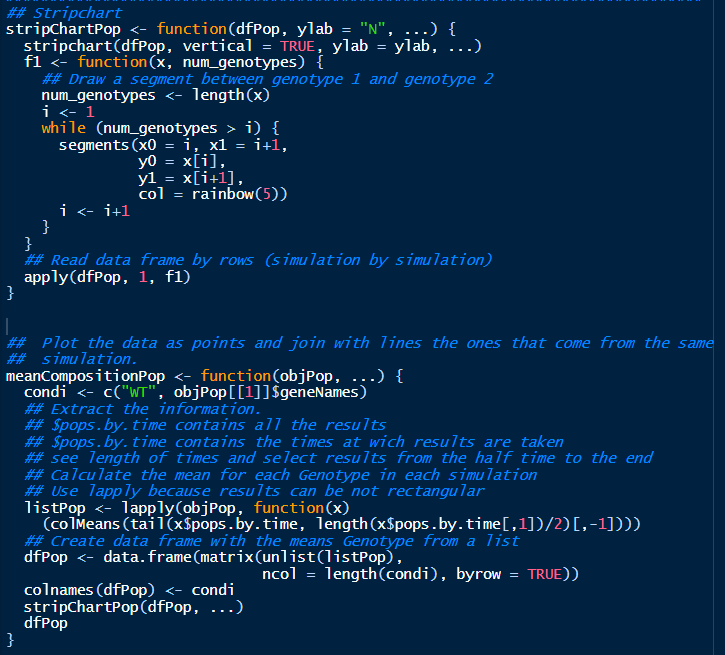
\includegraphics[width=0.6\linewidth]{img/stripchart_code.PNG}
        \caption{stripChartPop() and meanCompositionPop() code}
    \end{figure}
\end{frame}

\begin{frame}{Additional functions: graphical summary}
    \begin{figure}
    \centering
    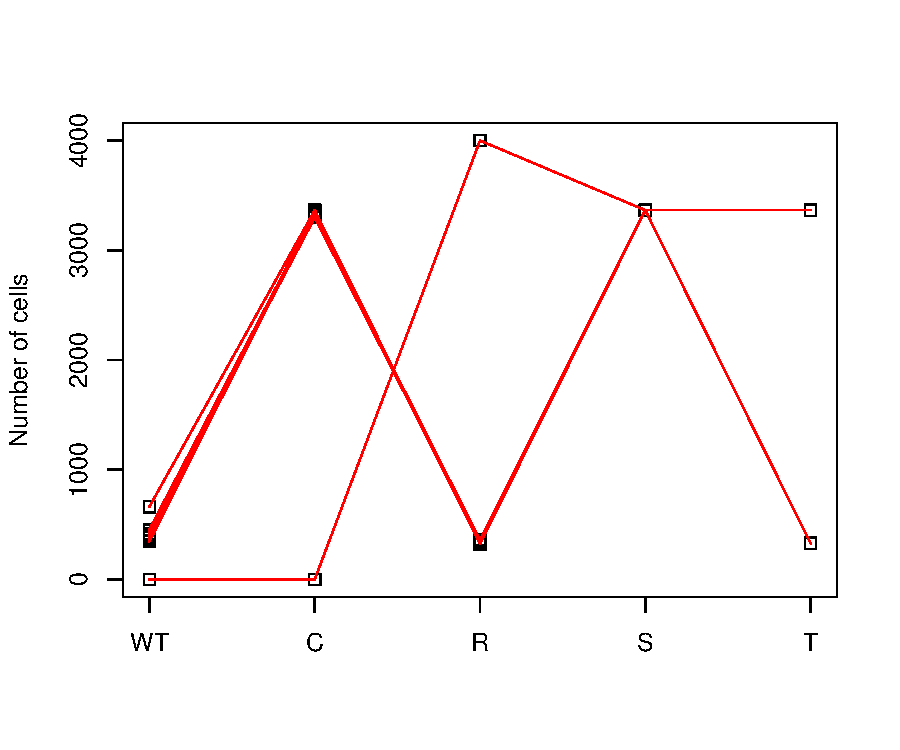
\includegraphics[width=0.8\linewidth]{img/stripchart_example.pdf}
    \caption{Example of the graphical summary of an oscillating trajectory}
    \end{figure}
\end{frame}

\subsection{Modification of the code}

\begin{frame}{Modification of the code}
	\begin{itemize}
		\item \textbf{Legend location}: plot.oncosimul and plotClonesSt
	\end{itemize}
    \begin{figure}
    \centering
    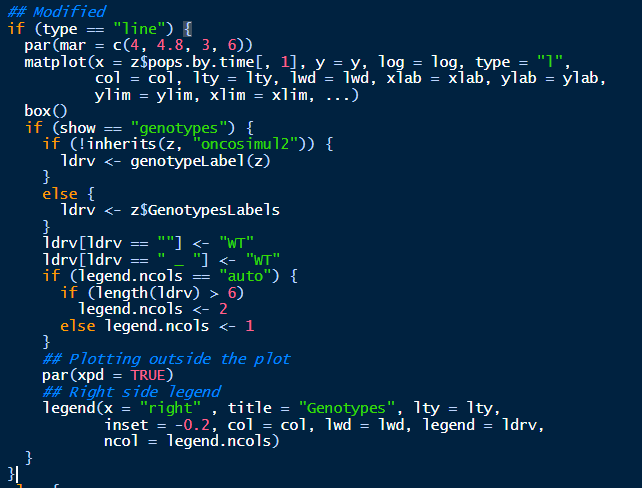
\includegraphics[width=0.7\linewidth]{img/plot_legend_outside.PNG}
    \caption{Par settings for placing the legend outside}
    \end{figure}
\end{frame}

\begin{frame}{Modification of the code}
	\begin{itemize}
		\item \textbf{Legend location}
	\end{itemize}
	\begin{columns}
		\begin{column}{0.5\textwidth}
			\begin{figure}
				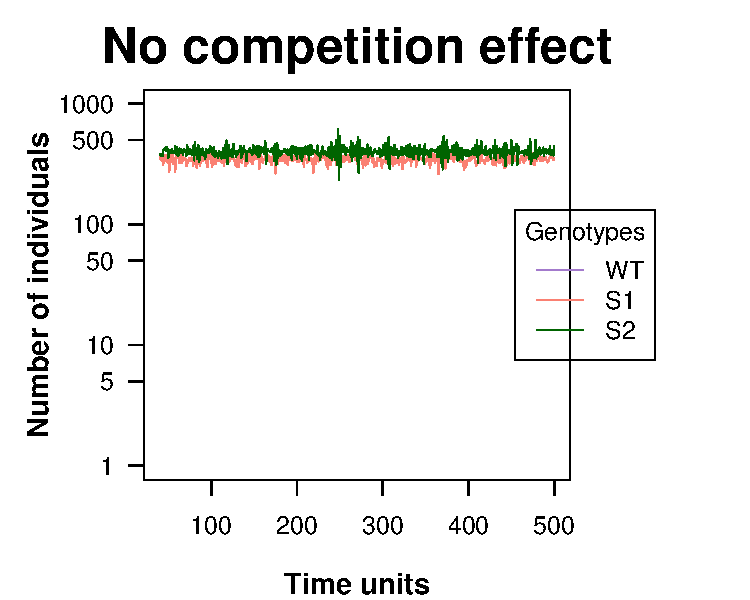
\includegraphics[width=0.95\linewidth]{img/line_example.pdf}
			\end{figure}
		\end{column}
		\begin{column}{0.5\textwidth}
			\begin{figure}
				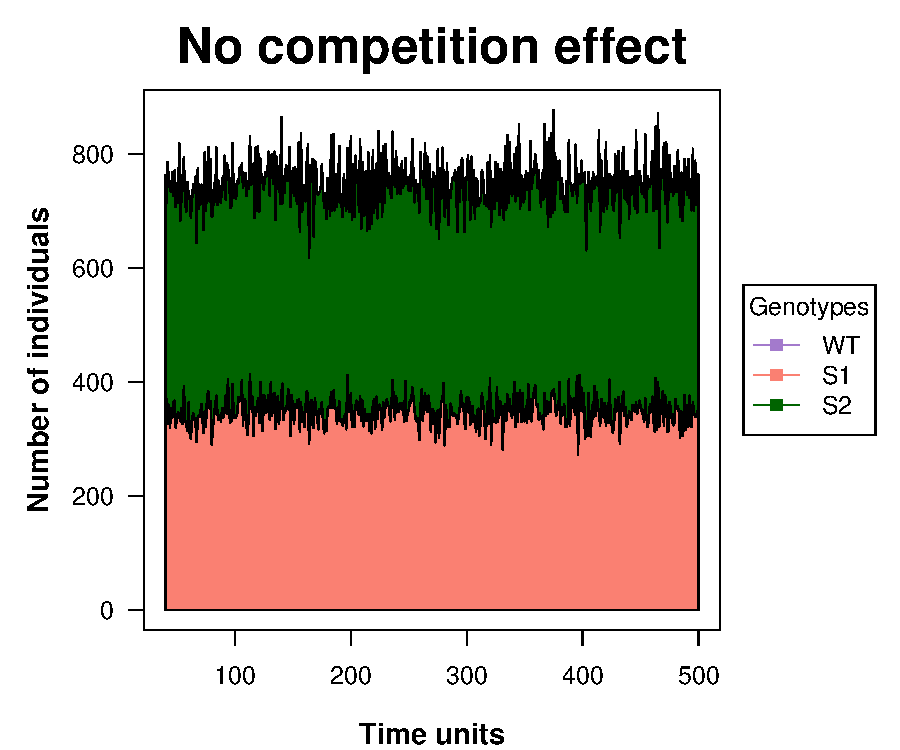
\includegraphics[width=0.95\linewidth]{img/stream_example.pdf}
			\end{figure}
		\end{column}
	\end{columns}
\end{frame}
